\documentclass[12pt]{article}
\usepackage{amsmath}
\usepackage{amssymb}
\usepackage{geometry}
\usepackage{enumerate}
\usepackage{natbib}
\usepackage{float}%稳定图片位置
\usepackage{graphicx}%画图
\usepackage[english]{babel}
\usepackage{a4wide}
\usepackage{indentfirst}%缩进
\usepackage{enumerate}%加序号
\usepackage{multirow}%合并行
\title{\large UM-SJTU JOINT INSTITUTE\\PHYSICS LABORATORY\\(VP241)\\\ \\\ \\\ \\\ \\\ \\\ \\\ \\\ \\\ \\\ \\\
LABORATORY REPORT\\\ \\\ EXERCISE 5\\\ RC, RL, and RLC Circuits \\\ \\\ \\\ \\\ \\\ }
\author{Name: Pan Chongdan \\ID: 516370910121\\Group: 6}
\date{Date: \today}

\begin{document}
\maketitle
\newpage
\section{Objectives}
\begin{enumerate}
\item Understand the physics of alternating-current circuits, in particular the processes of charging and discharging of capacitors.
\item Understand the phenomenon of electromagnetic induction in inductive elements, and other dynamic processes in $RC$,
$RL$, and $RLC$ series circuits.
\item Study the methods for measuring the amplitude-frequency and the phase-frequency characteristics of $RC$, $RL$, and $RLC$ series circuits.
\item Find the resonance frequency of a $RLC$ circuit as well as the quality factor of the circuit from the amplitude-frequency curve.
\end{enumerate}
\section{Theoretical Background}
Resistors, capacitors, and inductors are basic elements of electric circuits. Depending on a particular arrangement of these elements, $RC$, $RL$, $RLC$ alternating-current (AC) circuits may display various features, including transient, steady state, and resonant behavior.
\subsection{Transient Processes in $RC,RL,RLC$ Series Circuits}
\subsubsection{$RC$ Series Circuits}
In a $RC$ circuit, the process of charging or discharging of the capacitor is an example
of a transient process.
\begin{figure}[H]
\centering
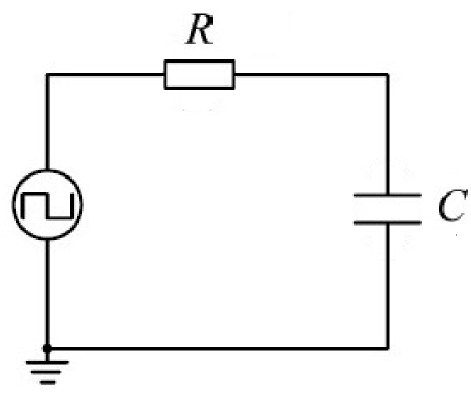
\includegraphics[scale=0.4]{P1.jpg}
\caption{$RC$ series circuit}.
\end{figure}
Figure 1 shows a $RC$ series circuit in which a square-wave signal is used as the source signal. In the first half of the cycle, the square-wave voltage is $U_(t)=\varepsilon$ and it charges the capacitor. In the second half-cycle, the square-wave voltage is 0, and the capacitor discharge through the resistor. The loop equation for the charging process is 
\begin{equation}
RC\frac{\mathrm{d}U_C}{\mathrm{d}t}+U_c=\varepsilon
\end{equation}
With the initial condition $U_C(t=0)=0,$ the solution of Eq.(1) can be found as
$$U_C=\varepsilon(1-e^{-\frac{t}{RC}})$$
$$U_R=iR=\varepsilon e^{-\frac{t}{RC}}$$
Hence the voltage across the capacitor $U_C$ increases exponentially with time $t$, whereas the voltage on the resistor $U_R$ decreases exponentially with time. The curves $U(t)$, $U_C(t)$,
and $U_R(t)$ are shown in Figure 2
\begin{figure}[H]
\centering
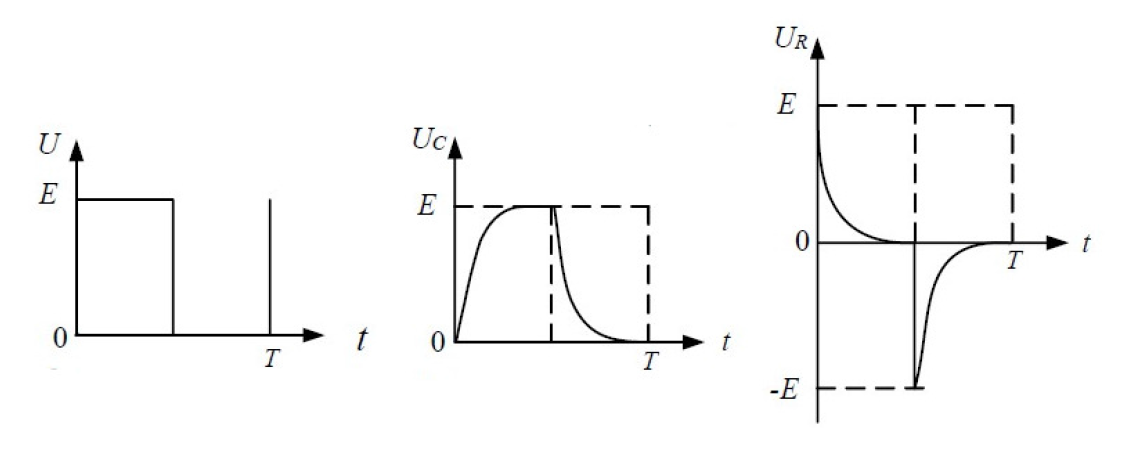
\includegraphics[scale=0.4]{P2.jpg}
\caption{Charging and discharging curves for a $RC$ series circuit.}
\end{figure}
\par For the discharging process, the loop rule gives
\begin{equation}
RC\frac{\mathrm{d}U_c}{\mathrm{d}t}+U_C=0
\end{equation}
The solution of Eq.(2), with the initial condition $U_C=(t=0)=\varepsilon$, is 
$$U_C=\varepsilon e^{-\frac{t}{RC}}$$
and consequently,
$$U_R=iR=-\varepsilon e^{-\frac{t}{RC}}$$
where the magnitudes of both $U_C$ and $U_R$ decrease exponentially with time. Since $RC=\tau$ has the units of time, it is called the time constant of the circuit, and characterizes the dynamics of the transient process. There is another characteristics related to the time constant, easier to measure in experiments, which is called the half-life period $T_\frac{1}{2}$. The half-life period is the time needed for $U_C$ to decrease to a half of the initial value (or
increase to a half of the terminal value), and may be also used to characterize the dynamics of the transient process. Both quantities, in the process with exponential dynamics discussed above, are related by the equation
$$T_{\frac{1}{2}}=\tau\ln2\approx0.693\tau$$
\subsection{$RL$ Series Circuit}
A similar analysis can be carried out for a $RL$ series circuit. In this case,
$$\tau-\frac{L}{R},T_{\frac{1}{2}}=\frac{L}{R}\ln2$$
\subsection{$RLC$ Series Circuit}
First, let us discuss the situation when a power source is suddenly plugged into a $RLC$
circuit. Then the voltage across the capacitor satisfies the differential equation
\begin{equation}
LC\frac{\mathrm{d^2}U_C}{\mathrm{d}t^2}+RC\frac{\mathrm{d}U_C}{\mathrm{d}t}+U_C=\varepsilon
\end{equation}
following again from the loop rule. Dividing both sides of the equation by LC and
introducing the symbols
\begin{equation}
\beta=\frac{R}{2L},\omega_0=\frac{1}{\sqrt{LC}}
\end{equation}
Eq.(3) can be written as 
\begin{equation}
\frac{\mathrm{d^2}U_C}{\mathrm{d}t^2}+2\beta\frac{\mathrm{d}U_C}{\mathrm{d}t}+\omega_0^2U_C=\omega_0^2\varepsilon
\end{equation}
Note that Eq. (5) is an inhomogeneous differential equation and it is mathematically equivalent to the equation of motion of a damped harmonic oscillator with a constant driving force. Therefore, the complementary homogeneous equation is fully analogous
to the equation of motion of a damped harmonic oscillator, with $\beta$ being the damping coefficient, and $\omega_0$ the natural angular frequency. Moreover, after a specific solution to the inhomogeneous equation is found, a unique solution to the initial value problem consisting of Eq.(5) and the initial conditions
\begin{equation}
U_C=(t=0)=0,\frac{\mathrm{d}U_C}{\mathrm{d}t}(t=0)=0
\end{equation}
can be found.
\par Exactly as for mechanical oscillations, depending on the relation between $\beta$ and $\omega_0$,
there are three regimes, as implied by the solution of the complementary homogeneous
equation:
\begin{enumerate}
\item If $\beta^2-\omega_0^2<0$ (weak damping), the system is in the underdamped regime and the
solution to the initial value problem is of the form
$$U_C=\varepsilon-\varepsilon e^{-\beta t}(\cos\omega t+\frac{\beta}{\omega}\sin t)$$
where $\omega=\sqrt{\omega_0^2-\beta^2}$
\item If $\beta^2-\omega_0^2<0$ (strong damping), the system is in the overdamped regime and the
solution to the initial value problem is of the form
$$U_C=\varepsilon-\frac{\varepsilon}{2\gamma}e^{-\beta t}[(\beta+\gamma)e^{\gamma t}-(\beta-\gamma)e^{-\gamma t}]$$
where $\omega=\sqrt{\beta^2-\omega_0^2}$
\item f $\beta^2-\omega_0^2=0$ the system is said to be critically damped, and 
\begin{equation}
U_C=\varepsilon-\varepsilon(1+\beta t)e^{-\beta t}
\end{equation}
\end{enumerate}
When the circuit reaches a steady state, the power source is suddenly removed ($\varepsilon=0$).
The differential equation for the discharging process is similar to that of the charging
process, and there are also three regimes of the process.
\par The above discussion is valid for an ideal circuit and a step-signal source with zero
internal resistance. In the experiment, the ideal system is replaced by a square-wave
source with a small internal resistance. The period of the square-signal must be much
greater than the time constant of the circuit. Note that, according to the above equations,
the voltage across the capacitor $U_C$ will finally reach $\varepsilon$ regardless of the regime (Figure
5, charging phase).
\begin{figure}[H]
\centering
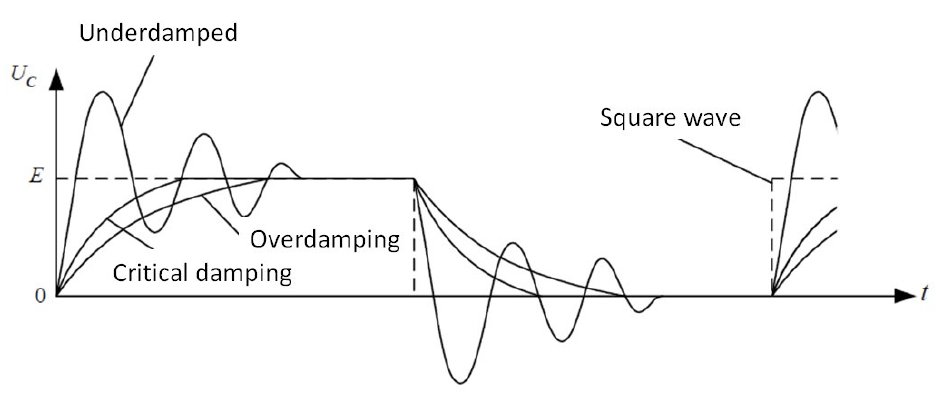
\includegraphics[scale=0.4]{P3.jpg}
\caption{Three different regimes of transient processes in a $RLC$ series circuit.}
\end{figure}
\subsection{$RC,RL$ Steady State Circuits}
When a sinusoidal alternating input voltage is provided to a $RC$ (or $RL$) series circuit,
the amplitude and the phase of the voltage across the capacitor and the resistor will change
with the frequency of the input voltage. Then the amplitude vs. frequency relation and
the phase vs. frequency relation can be obtained by measuring the voltage across the
elements in the circuit for different input signal frequencies
$$\varphi=\tan^{-1}(\frac{U_L}{U_R})=\tan^{-1}(\frac{\omega L}{R}),\varphi=(-\frac{U_C}{U_R})=\tan^{-1}(-\frac{1}{\omega RC})$$
\subsection{$RLC$ Resonant Circuit}
\subsubsection{$RLC$ Series Circuit}
\begin{figure}[H]
\centering
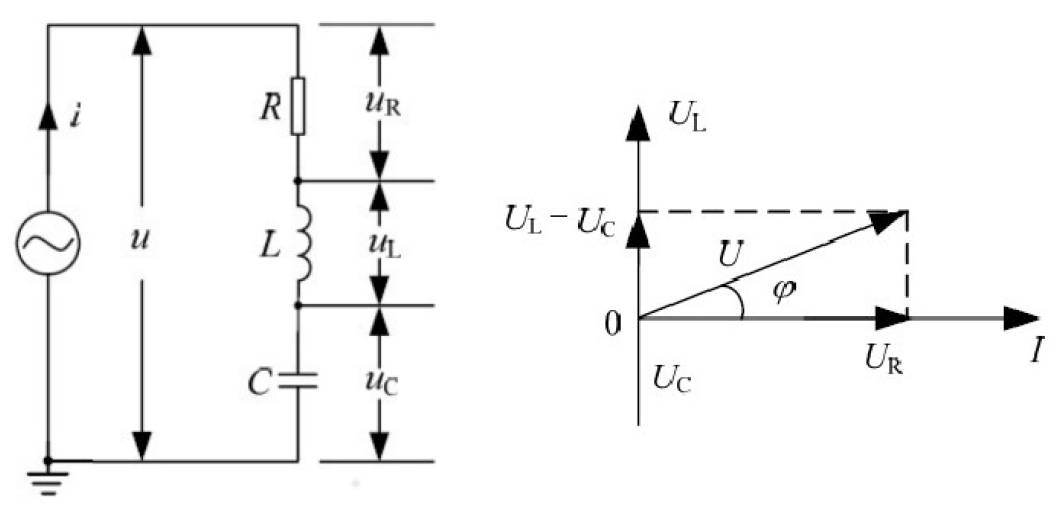
\includegraphics[scale=0.4]{P4.jpg}
\caption{$RLC$ series circuit.}
\end{figure}
A generic $RLC$ series circuit is shown in Figure 4. The impedance and the phase difference in the $RLC$ circuit can be calculated by using the phasers technique. Representing the current I by a vector along the horizontal axis, the phase differences between the current and the voltages across the resistor, coil, and capacitor are
$$\varphi_R=0,\varphi_L=\frac{\pi}{2},\varphi=-\frac{\pi}{2}$$
respectively. The corresponding voltage amplitudes across the elements are
$$U_R=IZ=IZ,U_Z=IZ_L=I\omega L,U_C=IZ_C=\frac{I}{\omega C}$$
Hence the voltage amplitude are 
\begin{equation}
U=\sqrt{U_R^2+(U_L-U_C)^2}\quad\mathrm{or}\quad U=I\sqrt{R^2+(\omega L-\frac{1}{\omega C})^2}
\end{equation}
and the total impedance
\begin{equation}
Z=\sqrt{R^2+(\omega L-\frac{1}{\omega C})^2}
\end{equation}
with the phase difference between the current and the voltage in the circuit
$$\varphi=\tan^{-1}(\frac{U_L-U_C}{U_R})=\tan^{-1}(\frac{\omega L-\frac{1}{\omega C}}{R})$$
\subsection{Resonance}
If the frequency of the input signal provided by the source satisfies the condition
$$\omega_0L=\frac{1}{\omega_0C},\quad\mathrm{or,equivalently,}\quad\omega_0=\frac{1}{\sqrt{LC}}$$
the total impedance will reach a minimum, $Z_0=R$. Note that the resistance R in a real
circuit includes the internal resistance and all kinds of alternating-current power losses,
so its actual value will be greater than the theoretical one.
When the current reaches its maximum, $I_m=\frac{U}{R}$, the circuit is said to be at resonance. The frequency
$$f_0=\frac{\omega_0}{2\pi}=\frac{1}{2\pi\sqrt{LC}}$$
at which the resonance phenomenon occurs, is called the resonance frequency.
\begin{figure}[H]
\centering
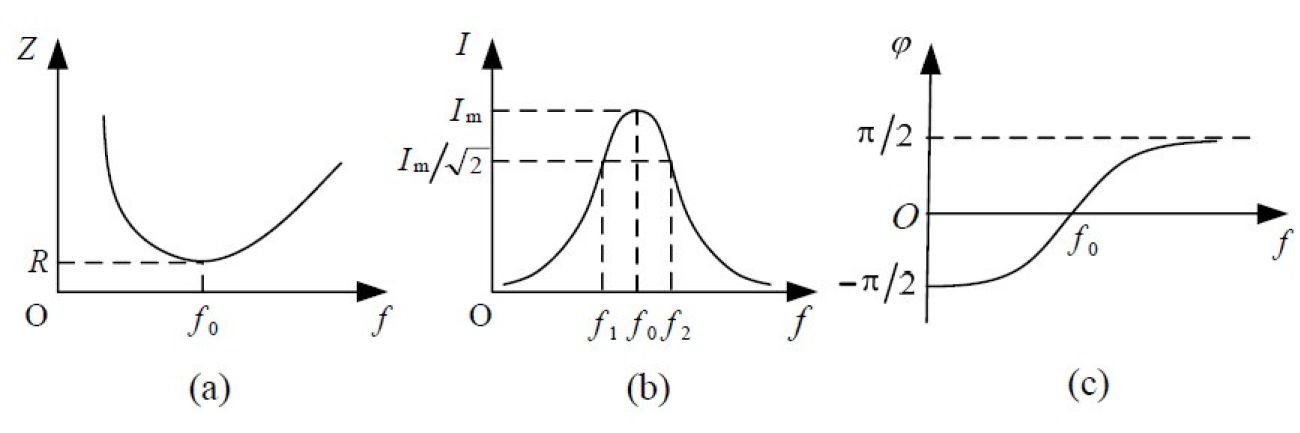
\includegraphics[scale=0.4]{P5.jpg}
\caption{The impedance, the current and the phase difference as functions of the frequency for a $RLC$ series circuit (generic sketches).}
\end{figure}
\par The total impedance $Z$, the current $I$, and the phase difference $\varphi=\varphi_u-\varphi_i$ all depend
on the frequency, with generic shapes of the three curves shown in Figure 5. According
to Eqs. (8) and (9), when the frequency is low $(f<f_0,\frac{1}{\omega C}>\omega L)$, then $\varphi<0$.
In this situation the total voltage lags behind the current and the circuit is said to be capacitive.
When the circuit is resonant $(f<f_0,\frac{1}{\omega C}=\omega L)$, then $\varphi=0$ and the voltages
across the capacitor and the inductor should be equal. The circuit is said to be resistive.
\subsection{Quality Factor in Resonant Circuits}
Since $I_m=\frac{U}{R},$ the voltages across the resistor, the inductor, and the capacitor are
$$U_R=I_m R=U$$
$$U_L=I_M Z_L=\frac{U}{R}\omega L$$
$$U_C=I_M Z_C=\frac{U}{R}\frac{1}{\omega_0 C}=U_L$$
respectively. For a circuit driven at the resonance frequency, the ratio of $U_L$ or $U_C$ to $U$ is called the quality factor $Q$ of a resonant circuit
$$Q=\frac{U_L}{U}=\frac{\omega_0 L}{R}\quad\mathrm{or}\quad Q=\frac{U_C}{U}=\frac{1}{\omega_0 RC}$$
When the total voltage is fixed, the greater $Q$ is, the greater $U_L$ and $U_C$ are. The value
of $Q$ can be used to quantify the efficiency of resonant circuits.
\par The quality factor can be also found as 
$$Q=\frac{f_0}{f_2-f_1}$$
where $f_1$ and $f_2$ are two frequencies such that $I(f_1)=I(f_2)=\frac{I_m}{\sqrt{2}}$
\section{Apparatus}
The measurement setup consists of the following main elements: a signal generator, an
oscilloscope, a digital multimeter, a wiring board, a fixed resistor $100\Omega(2W)$, a variable
resistor $2k\Omega(2W)$, two capacitors $0.47\mu F$ and $0.1\mu F$, as well as two inductors ($10mH$
and $33mH$).
\section{Measurement Procedure}
\subsection{$RC,RL$ Series Circuit}
\begin{enumerate}
\item I chose a capacitor and an inductor to assemble a circuit with the fixed-resistance $100\Omega$ resistor, adjusted the output frequency of the square-wave signal provided by the signal generator, and observed the change of the waveform when the time constant is smaller or greater than the period of the square wave. Then I chose the frequency that allows the capacitor to fully charge/discharge and use the PRINT function of the oscilloscope to store the waveforms.
\item I adjusted display parameters of the oscilloscope and measured $T_{\frac{1}{2}}$ for the studied circuits. In the report, I calculate the time constant and compare it with the theoretical value. 
\end{enumerate}
\subsection{$RLC$ Series Circuit}
\begin{enumerate}
\item I chose a capacitor and an inductor to assemble a $RLC$ series circuit with the variable resistor and observed the waveform of the capacitor voltage in the underdamped, critically damped, and overdamped regimes. I used the PRINT function of the oscilloscope to store the waveforms.
\item I adjusted the variable resistor to the critically damped regime. According to the
definition of the half-life period $T_{\frac{1}{2}}$, we have $\beta T_{\frac{1}{2}}=1.68$. By finding the value of
$T_{\frac{1}{2}}$, the time constant can be found as $\tau=\frac{1}{\beta}=T_{\frac{1}{2}}/1,68$. In the report, my result
with the theoretical value.
\end{enumerate}
\subsection{$RLC$ Resonant Circuit}
I applied a sinusoidal input voltage $U_i$ to the $RLC$ series circuit, changed the frequency,
then observed the change of the voltage $U_R$ for a fixed resistor $R$, as well as the phase
difference between $U_R$ and $U_i$. I measured how UR changes with $U_i$ and calculated the phase
difference according to Figure 4. The graphs $\frac{I}{I_m}$ vs. $\frac{f}{f_0}$ and $\varphi$ vs. $\frac{f}{f_0}$ are plotted in the report. I also estimated the resonance frequency and calculate the quality factor $Q$.
\section{Results and Calculations}
\subsection{$RC$ Series Circuit}
\begin{table}[H]
\centering
\begin{tabular}{|c|c|}
\hline
$R$&$98.55\pm0.01[\Omega]$\\ \hline
$f$&$4000\pm0.001[\mathrm{Hz}]$\\ \hline
$\varepsilon$&$4.00\pm0.001[\mathrm{V}]$\\ \hline
$C$&$100.52\pm0.01[\mathrm{nF}]$\\ \hline
$T_{1/2}$&$7.000\pm0.001[\mu s]$\\ \hline
\end{tabular}
\caption{$T_{1/2}$ measurement data for a $RC$ series circuit}
\end{table}
\begin{figure}[H]
\centering
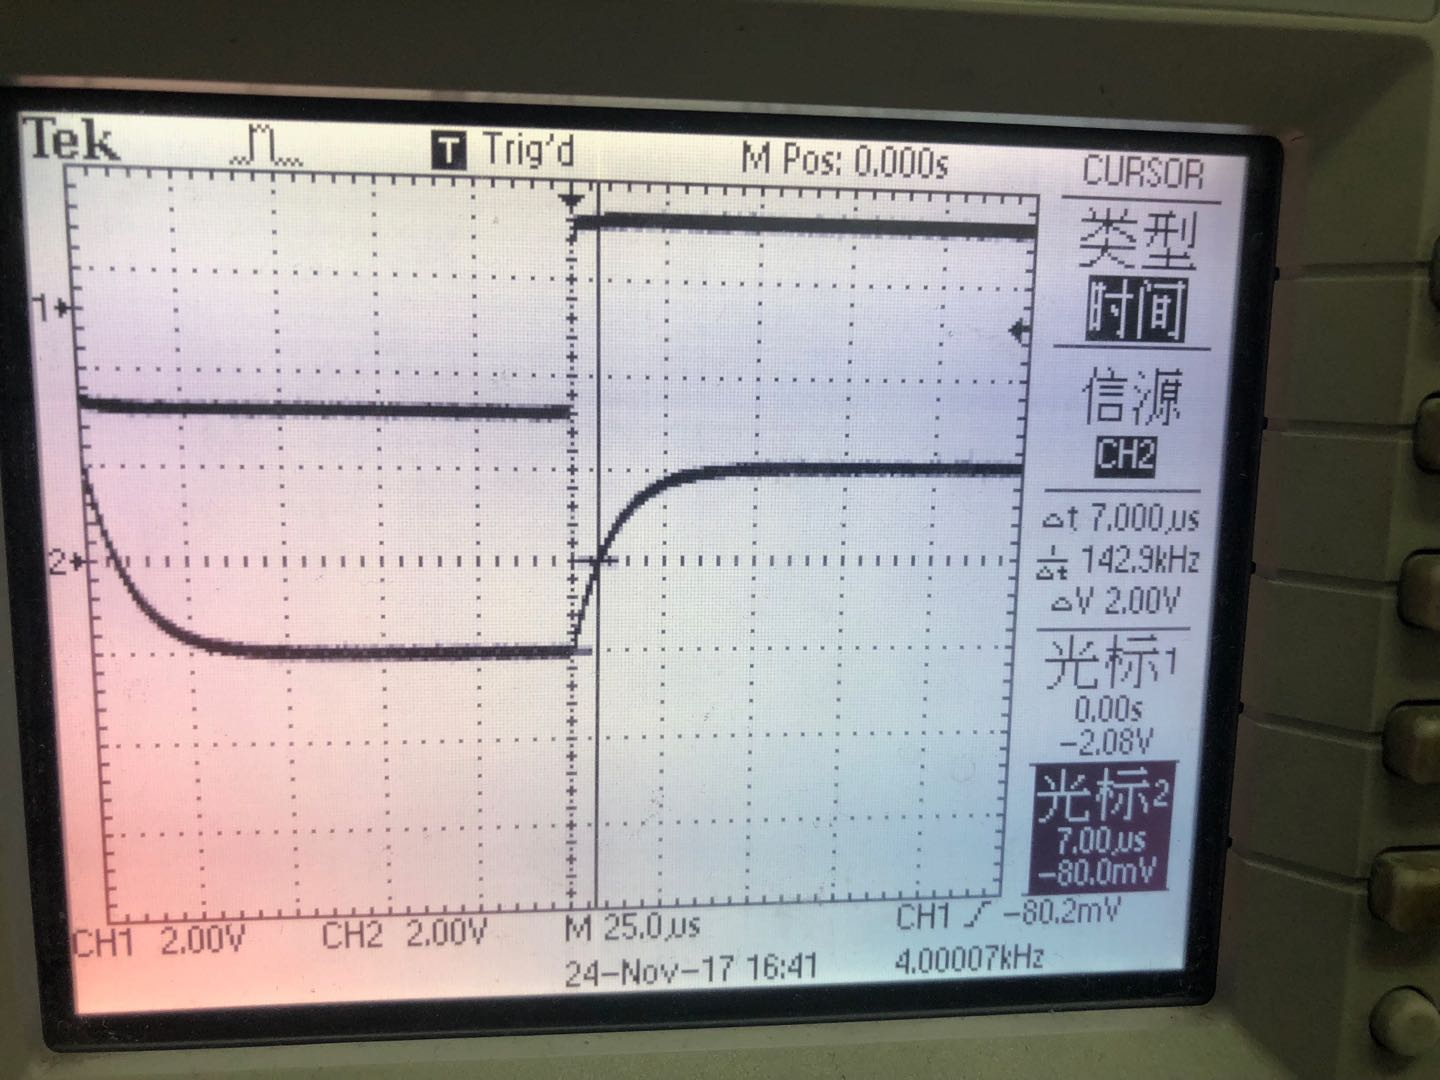
\includegraphics[scale=0.2]{P6.jpg}
\caption{Figure of RC series circuit's waveform}
\end{figure}
The theoretical value of time constant:
$$\tau_{th}=RC=98.55\cdot100.52=9.906\pm1.41\cdot10^{-3}[\mu s]$$
\par The experimental value of time constant:
$$\tau_{ex}=\frac{T_{1/2}}{\ln2}=10.10\pm1.44\cdot10^{-3}[\mu s]$$
\subsection{$RL$ Series Circuit}
\begin{table}[H]
\centering
\begin{tabular}{|c|c|}
\hline
$R$&$98.55\pm0.01[\Omega]$\\ \hline
$f$&$500\pm0.001[\mathrm{Hz}]$\\ \hline
$\varepsilon$&$4.08\pm0.001[\mathrm{V}]$\\ \hline
$L$&$0.01\pm0[\mathrm{[H]}$\\ \hline
$T_{1/2}$&$64.00\pm0.001[\mu s]$\\ \hline
\end{tabular}
\caption{$T_{1/2}$ measurement data for a RL series circuit}
\end{table}
The theoretical value of time constant:
$$\tau_{th}=\frac{L}{R}=\frac{0.01}{98.55}=101.5\pm0.01[\mu s]$$
\par The experimental value of time constant:
$$\tau_{ex}=\frac{T_{1/2}}{\ln2}=92.33[\mu s]$$
\subsection{$RLC$ Series Circuit}
\begin{table}[H]
\centering
\begin{tabular}{|c|c|}
\hline
$L$&$0.01\pm0[\mathrm{[H]}$\\ \hline
$C$&$100.52\pm0.01[\mathrm{nF}$\\ \hline
$\varepsilon$&$4.48\pm0.001[\mathrm{V}]$\\ \hline
$f$&$200\pm0.001[\mathrm{Hz}]$\\ \hline
$\beta t$&1.68\\ \hline
$T_{1/2}$&$48.00\pm0.001[\mu s]$\\ \hline
\end{tabular}
\caption{$T_{1/2}$ measurement data for a critically damped $RLC$ series circuit}
\end{table}
\par The experimental value of time constant:
$$\tau_{ex}=\frac{T_{1/2}}{\ln2}=69.25\pm1.44\cdot10^{-3}[\mu s]$$
\begin{figure}[H]
\centering
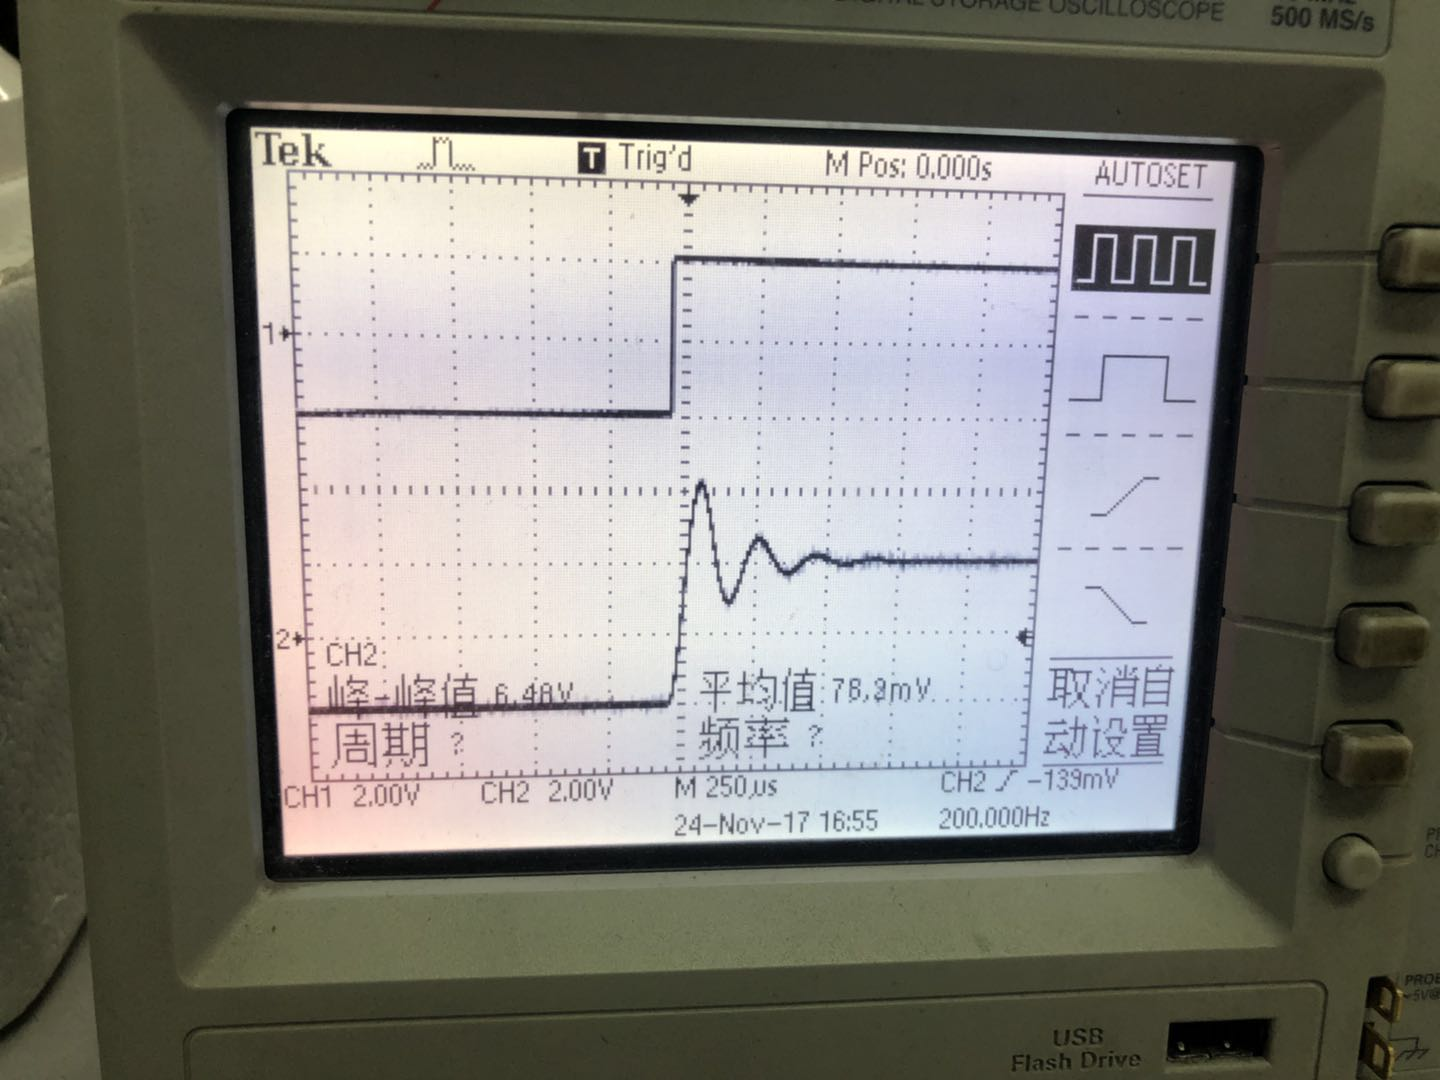
\includegraphics[scale=0.25]{P7.jpg}
\caption{Figure for underdamped regime waveform.}
\end{figure}
\begin{figure}[H]
\centering
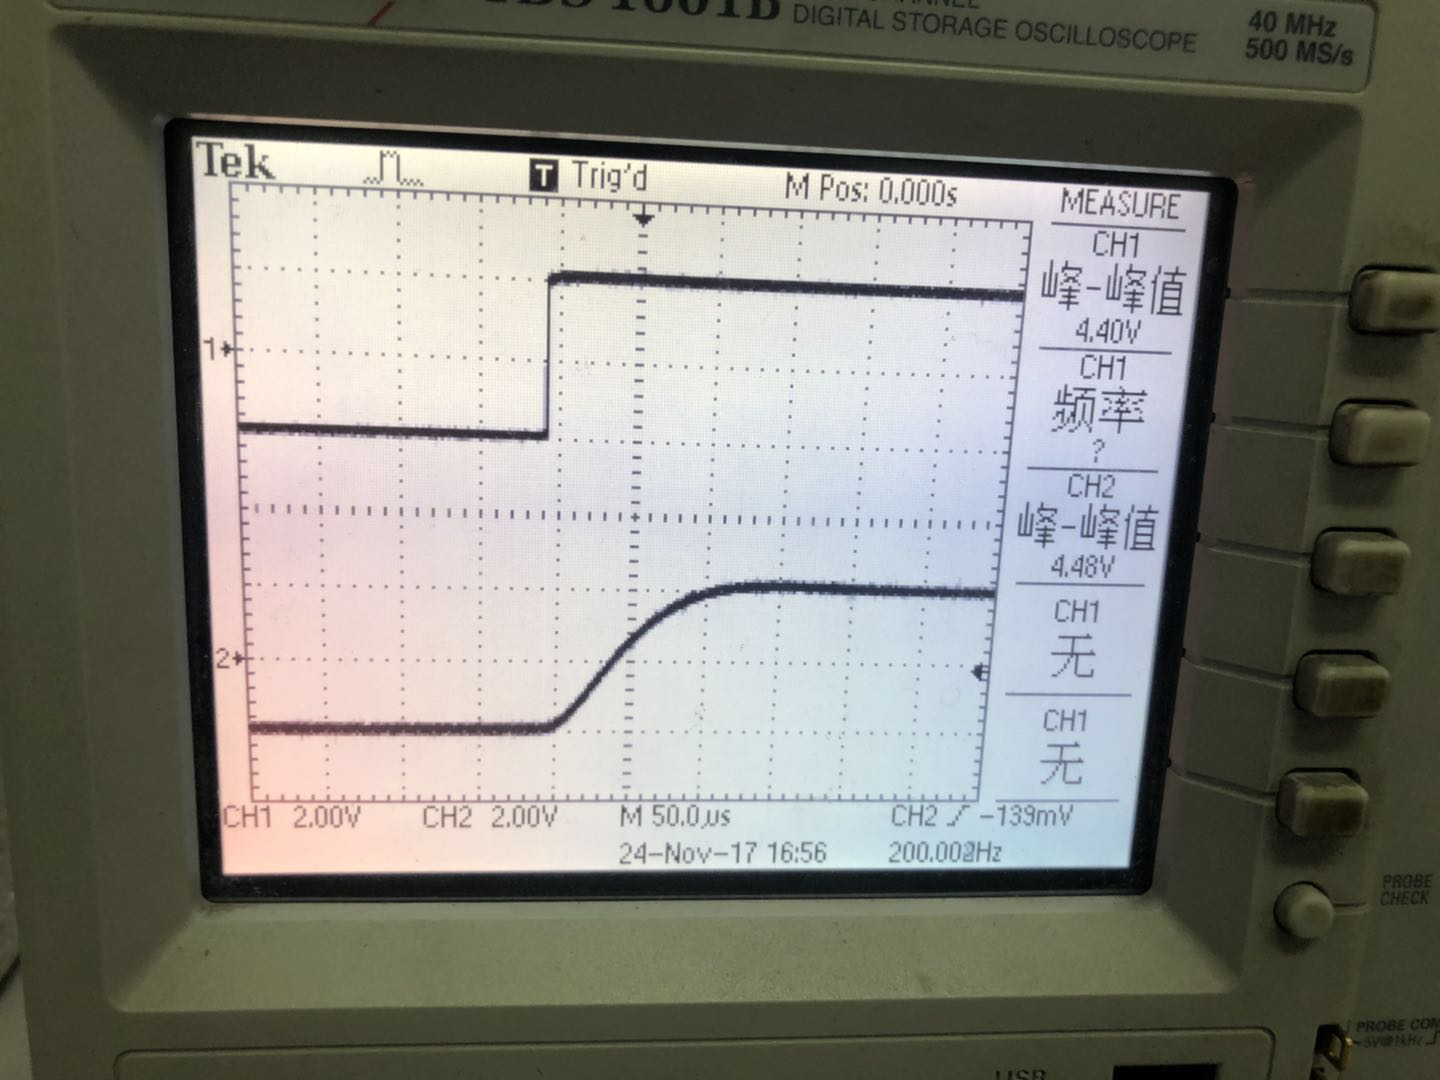
\includegraphics[scale=0.25]{P8.jpg}
\caption{Figure for critically damped regime waveform.}
\end{figure}
\begin{figure}[H]
\centering
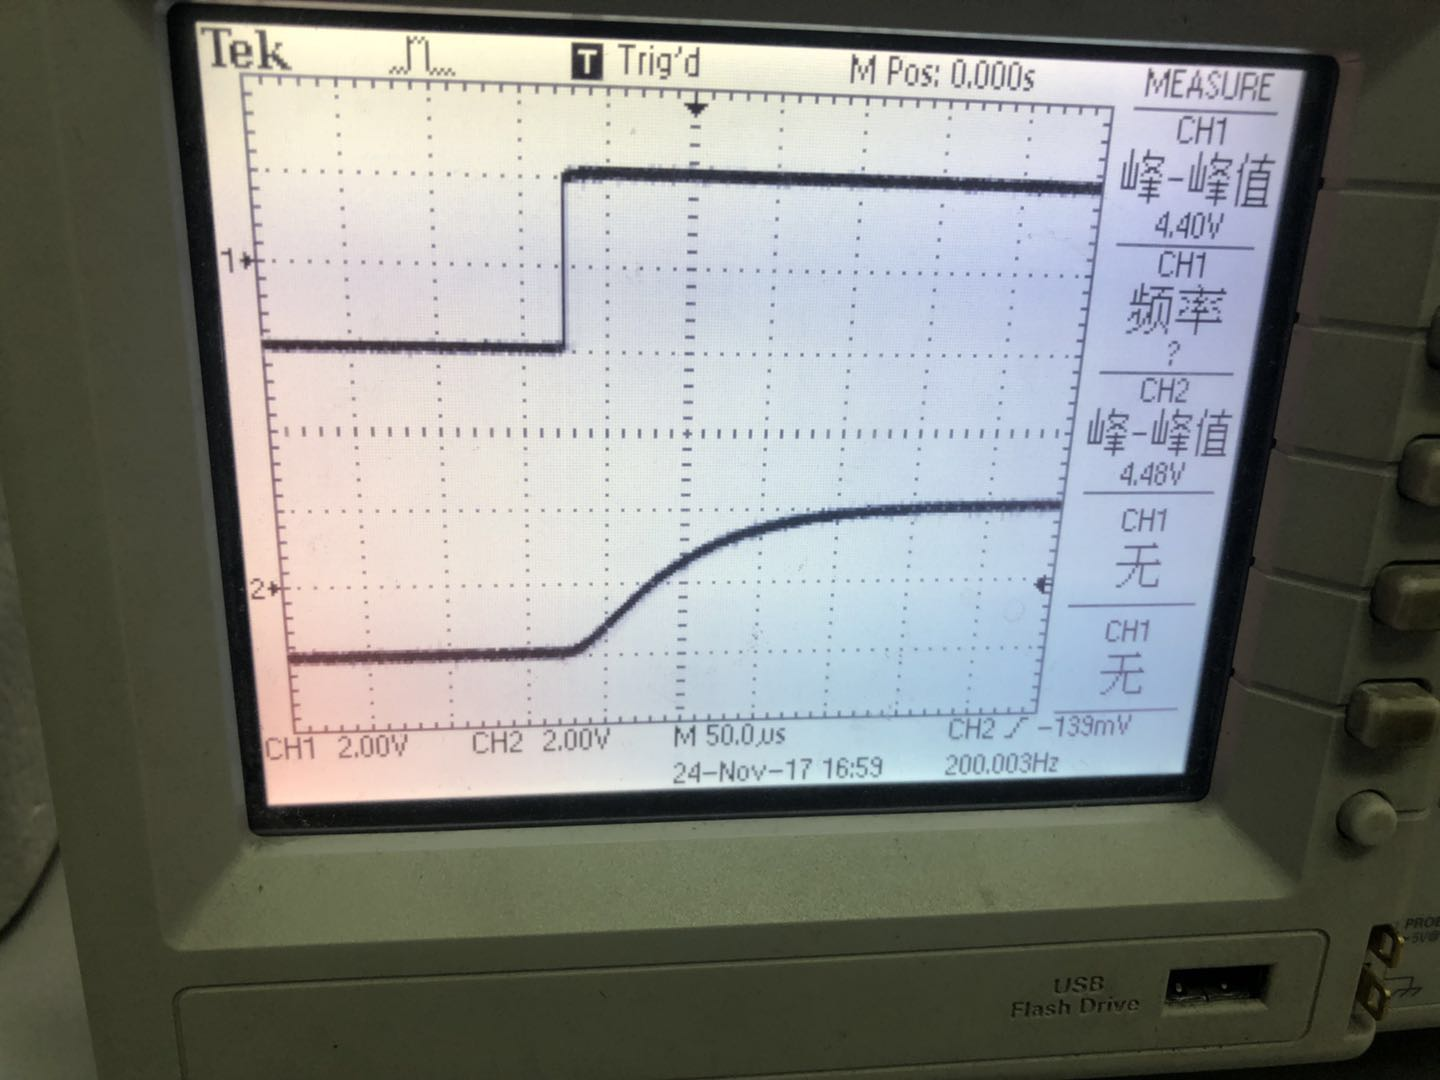
\includegraphics[scale=0.25]{P9.jpg}
\caption{Figure for overdamped regime waveform.}
\end{figure}
\subsection{$RLC$ Resonant Circuit}
\begin{table}[H]
\centering
\begin{tabular}{|c|c|c|}
\hline
$R$   & \multicolumn{2}{c|}{$98.55\pm0.01[\Omega]$} \\ \hline
$L$   & \multicolumn{2}{c|}{$0.01\pm0[\mathrm{[H]}$} \\ \hline
$C$   & \multicolumn{2}{c|}{$100.52\pm0.01[\mathrm{nF}$} \\ \hline
$f_0$   & \multicolumn{2}{c|}{$5000\pm0.001[\mathrm{Hz}]$} \\ \hline
$\varepsilon$   & \multicolumn{2}{c|}{$4.24\pm0.001[\mathrm{V}]$} \\ \hline
   &$U_R[V]\pm0.001[V]$           & $f[\mathrm{Hz}]\pm0.001[\mathrm{Hz}]]$          \\ \hline
1  & 0.56      & 1000      \\ \hline
2  & 0.64      & 1500      \\ \hline
3  & 0.80      & 2000      \\ \hline
4  & 1.04      & 2500      \\ \hline
5  & 1.36      & 3000      \\ \hline
6  & 1.76      & 3500      \\ \hline
7  & 2.48      & 4000      \\ \hline
8  & 2.88      & 4250      \\ \hline
9  & 3.44      & 4500      \\ \hline
10 & 3.84      & 4750      \\ \hline
11 & 3.92      & 5000      \\ \hline
12 & 3.76      & 5250      \\ \hline
13 & 3.44      & 5500      \\ \hline
14 & 3.12      & 5750      \\ \hline
15 & 2.72      & 6000      \\ \hline
16 & 2.16      & 6500      \\ \hline
17 & 1.84      & 7000      \\ \hline
18 & 1.60      & 7500      \\ \hline
19 & 1.36      & 8000      \\ \hline
20 & 1.28      & 8500      \\ \hline
21 & 1.20      & 9000      \\ \hline
\end{tabular}
\caption{Measurement data for the $U_R$ vs. $f$ dependence for a $RLC$ resonant circuit}
\end{table}
$$I_m=\frac{U_m}{R}=\frac{3.92}{98.55}=39.8\pm0.398[mA]$$
$$I_1=\frac{U_1}{R}=\frac{0.56}{98.55}=5.68\pm5.77\cdot10^{-2}[mA]$$
$$\frac{I_1}{I_m}=\frac{5.68}{39.8}=0.143$$
$$\frac{f_1}{f_0}=\frac{1000}{5000}=0.2$$
\begin{table}[H]
\centering
\begin{tabular}{|c|c|c|c|c|}
\hline
   &$U_R[V]\pm0.001[V]$  & $f[\mathrm{Hz}]\pm0.001[\mathrm{Hz}]]$  &$I/I_m$&$f/f_0$       \\ \hline
1  & 0.56      & 1000&0.143&0.20       \\ \hline
2  & 0.64      & 1500&0.163&0.30       \\ \hline
3  & 0.80      & 2000&0.204&0.40       \\ \hline
4  & 1.04      & 2500&0.265&0.50       \\ \hline
5  & 1.36      & 3000&0.347&0.60       \\ \hline
6  & 1.76      & 3500&0.449&0.70       \\ \hline
7  & 2.48      & 4000&0.633&0.80       \\ \hline
8  & 2.88      & 4250&0.735&0.85       \\ \hline
9  & 3.44      & 4500&0.877&0.90       \\ \hline
10 & 3.84      & 4750&0.980&0.95       \\ \hline
11 & 3.92      & 5000&1.000&1.00       \\ \hline
12 & 3.76      & 5250&0.959&1.05       \\ \hline
13 & 3.44      & 5500&0.877&1.10       \\ \hline
14 & 3.12      & 5750&0.796&1.15       \\ \hline
15 & 2.72      & 6000&0.694&1.20       \\ \hline
16 & 2.16      & 6500&0.551&1.30       \\ \hline
17 & 1.84      & 7000&0.469&1.40       \\ \hline
18 & 1.60      & 7500&0.408&1.50       \\ \hline
19 & 1.36      & 8000&0.347&1.60       \\ \hline
20 & 1.28      & 8500&0.327&1.70       \\ \hline
21 & 1.20      & 9000&0.306&1.80       \\ \hline
\end{tabular}
\caption{Calculated data for the $U_R$ vs. $f$ for a $RLC$ resonant circuit}
\end{table}
\subsubsection{Calculation of $Q$}
So the $f_1$ and $f_2$ according to the table is $4250$ and $6000\pm$ respectively. So the experimental value for quality factor is:
$$Q_{ex}=\frac{f_0}{f_2-f_1}=\frac{5000}{6000-4250}=2.857\pm2.38\cdot10^{-6}$$
The theoretical value of quality factor is 
$$Q_{th}=\frac{\sqrt{LC}}{RC}=\frac{\sqrt{0.01\cdot100.52}}{98.55\cdot100.52}=3.2\pm1.03\cdot10^{-8}$$
\begin{figure}[H]
\centering
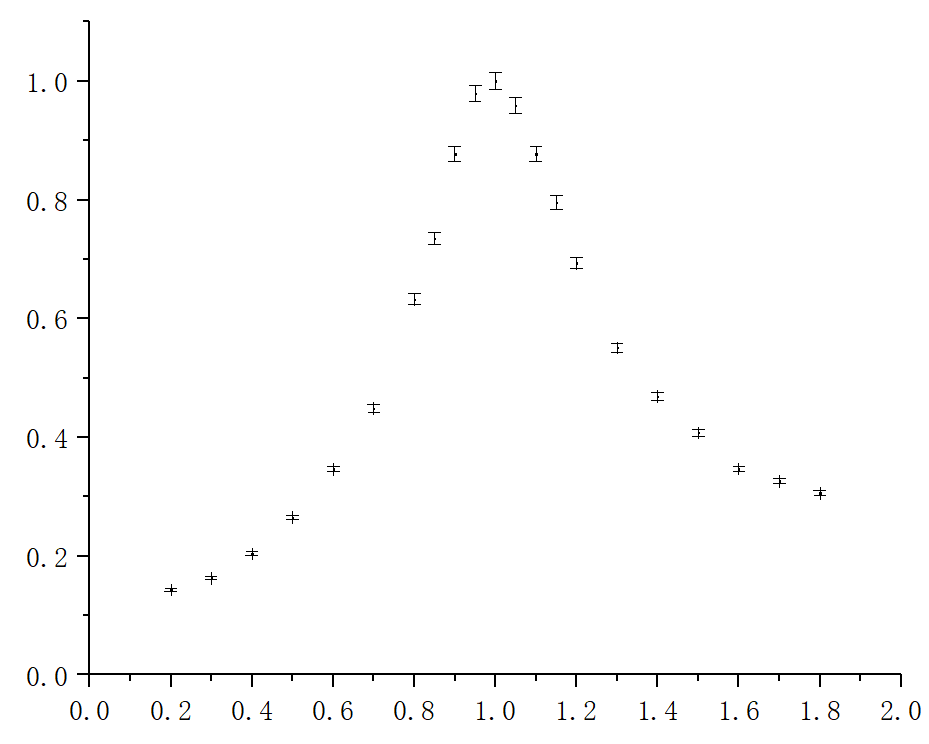
\includegraphics[scale=0.5]{P10.jpg}
\caption{Plot for $I/I_m$ vs. $f/f_0$}
\end{figure}
\subsection{Calculation of $\phi$}
For the theoretical value of $\phi$,
$$\phi_{th}=\arctan\frac{2\pi fL-\frac{1}{2\pi fC}}{R}=\arctan\frac{2\pi\cdot1000\cdot0.01-\frac{1}{2\pi\cdot1000\cdot100.52\cdot10^{-9}}}{98.55}=-1.506[\mathrm{rad}]$$
\begin{table}[H]
\centering
\begin{tabular}{|c|c|c|c|c|}
\hline
   &$U_R[V]\pm0.001[V]$  & $f[\mathrm{Hz}]\pm0.001[\mathrm{Hz}]]$  &$\phi_{th}$&$f/f_0$       \\ \hline
1  & 0.56      & 1000&-1.506&0.20       \\ \hline
2  & 0.64      & 1500&-1.469&0.30       \\ \hline
3  & 0.80      & 2000&-1.424&0.40       \\ \hline
4  & 1.04      & 2500&-1.367&0.50       \\ \hline
5  & 1.36      & 3000&-1.288&0.60       \\ \hline
6  & 1.76      & 3500&-1.170&0.70       \\ \hline
7  & 2.48      & 4000&-0.973&0.80       \\ \hline
8  & 2.88      & 4250&-0.820&0.85       \\ \hline
9  & 3.44      & 4500&-0.613&0.90       \\ \hline
10 & 3.84      & 4750&-0.342&0.95       \\ \hline
11 & 3.92      & 5000&-0.027&1.00       \\ \hline
12 & 3.76      & 5250& 0.277&1.05       \\ \hline
13 & 3.44      & 5500& 0.528&1.10       \\ \hline
14 & 3.12      & 5750& 0.716&1.15       \\ \hline
15 & 2.72      & 6000& 0.853&1.20       \\ \hline
16 & 2.16      & 6500& 1.031&1.30       \\ \hline
17 & 1.84      & 7000& 1.138&1.40       \\ \hline
18 & 1.60      & 7500& 1.208&1.50       \\ \hline
19 & 1.36      & 8000& 1.258&1.60       \\ \hline
20 & 1.28      & 8500& 1.294&1.70       \\ \hline
21 & 1.20      & 9000& 1.323&1.80       \\ \hline
\end{tabular}
\caption{Calculated data for the $\phi_{th}$ vs. $f$ for a $RLC$ resonant circuit}
\end{table}
\begin{figure}[H]
\centering
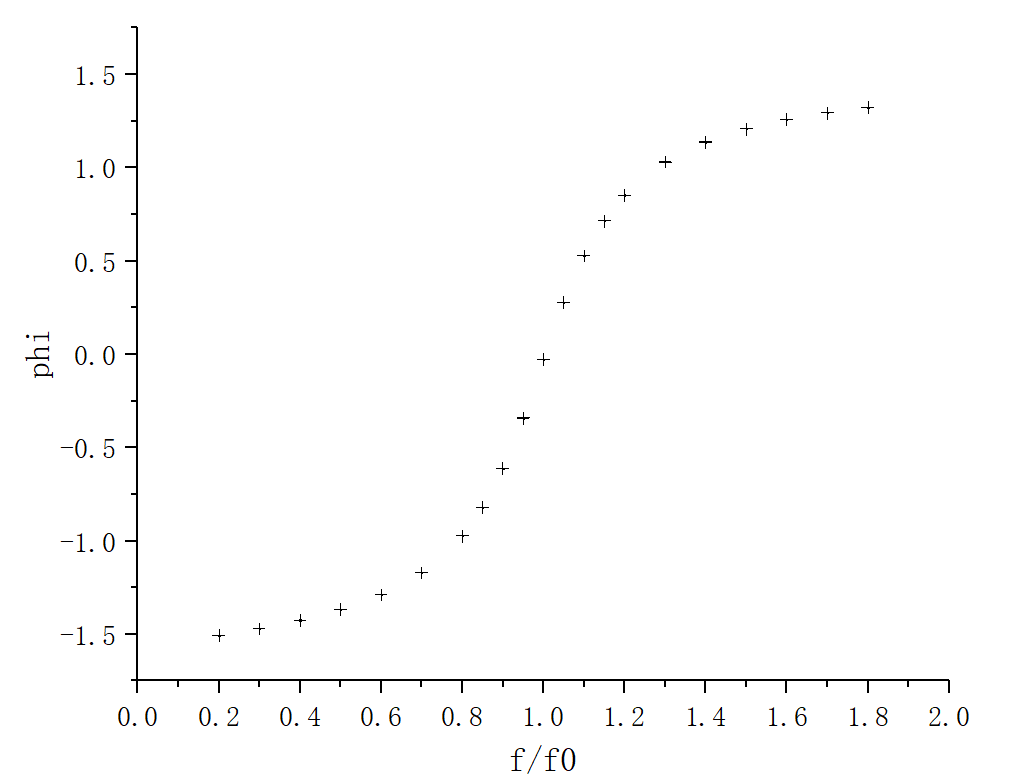
\includegraphics[scale=0.25]{P12.jpg}
\caption{Plot for $\phi_{th}$ vs. $f/f_0$}
\end{figure}
For the experimental value of $\phi$,
$$\phi_{ex}=\arccos\frac{U_R}{U_m}=-\arccos\frac{0.56}{3.92}=-1.427[\mathrm{rad}]$$
\begin{table}[H]
\centering
\begin{tabular}{|c|c|c|c|c|}
\hline
   &$U_R[V]\pm0.001[V]$  & $f[\mathrm{Hz}]\pm0.001[\mathrm{Hz}]]$  &$\phi_{ex}$&$f/f_0$       \\ \hline
1  & 0.56      & 1000&-1.427&0.20       \\ \hline
2  & 0.64      & 1500&-1.407&0.30       \\ \hline
3  & 0.80      & 2000&-1.365&0.40       \\ \hline
4  & 1.04      & 2500&-1.302&0.50       \\ \hline
5  & 1.36      & 3000&-1.217&0.60       \\ \hline
6  & 1.76      & 3500&-1.105&0.70       \\ \hline
7  & 2.48      & 4000&-0.885&0.80       \\ \hline
8  & 2.88      & 4250&-0.746&0.85       \\ \hline
9  & 3.44      & 4500&-0.500&0.90       \\ \hline
10 & 3.84      & 4750&-0.203&0.95       \\ \hline
11 & 3.92      & 5000& 0.000&1.00       \\ \hline
12 & 3.76      & 5250& 0.287&1.05       \\ \hline
13 & 3.44      & 5500& 0.500&1.10       \\ \hline
14 & 3.12      & 5750& 0.650&1.15       \\ \hline
15 & 2.72      & 6000& 0.804&1.20       \\ \hline
16 & 2.16      & 6500& 0.987&1.30       \\ \hline
17 & 1.84      & 7000& 1.082&1.40       \\ \hline
18 & 1.60      & 7500& 1.150&1.50       \\ \hline
19 & 1.36      & 8000& 1.217&1.60       \\ \hline
20 & 1.28      & 8500& 1.238&1.70       \\ \hline
21 & 1.20      & 9000& 1.260&1.80       \\ \hline
\end{tabular}
\caption{Calculated data for the $\phi_{ex}$ vs. $f$ for a $RLC$ resonant circuit}
\end{table}
\begin{figure}[H]
\centering
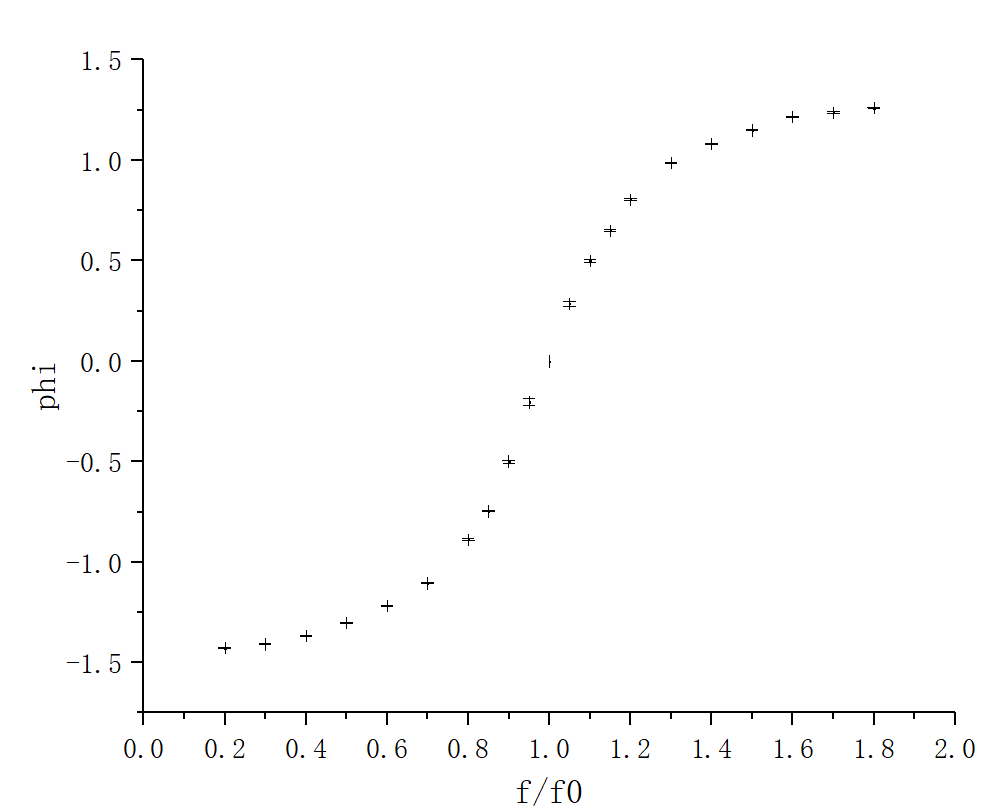
\includegraphics[scale=0.35]{P11.jpg}
\caption{Plot for $\phi_{ex}$ vs. $f/f_0$}
\end{figure}
\section{Uncertainty Analysis}
\subsection{$RC$ Series Circuit}
For uncertainty of $\tau_{th}$
$$u=\sqrt{(R\cdot u_C)^2+(c\cdot u_R)^2}=\sqrt{(98.55\cdot0.01)^2+(100.52\cdot0.01)}=1.41\cdot10^{-3}[\mu s]$$
\par The relative uncertainty:
$$u_r=\frac{u}{\tau_{th}}\cdot100\%=\frac{1.41\cdot10^{-3}}{9.906}\cdot100\%=0.01\%$$
\par For uncertainty of $\tau_{ex}$
$$u=u_T\cdot\frac{1}{\ln2}=\frac{0.001}{\ln2}=1.44\cdot10^{-3}[\mu s]$$
\par The relative uncertainty:
$$u_r=\frac{u}{\tau_{th}}\cdot100\%=\frac{1.44\cdot10^{-3}}{10.10}\cdot100\%=0.01\%$$
\subsection{$RL$ Series Circuit}
For uncertainty of $\tau_{th}$
$$u=\frac{u_RL}{R^2}=\frac{0.01\cdot0.01}{98.55^2}=0.01[\mu s]$$
\par The relative uncertainty:
$$u_r=\frac{u}{\tau_{th}}\cdot100\%=\frac{0.01}{101.5}\cdot100\%=0.01\%$$
\par For uncertainty of $\tau_{ex}$
$$u=u_T\cdot\frac{1}{\ln2}=\frac{0.001}{\ln2}=1.44\cdot10^{-3}[\mu s]$$
\par The relative uncertainty:
$$u_r=\frac{u}{\tau_{th}}\cdot100\%=\frac{1.44\cdot10^{-3}}{92.33}\cdot100\%=0.001\%$$
\subsection{$RLC$ Series Circuit}
For uncertainty of $\tau_{ex}$
$$u=u_T\cdot\frac{1}{\ln2}=\frac{0.001}{\ln2}=1.44\cdot10^{-3}[\mu s]$$
\par The relative uncertainty:
$$u_r=\frac{u}{\tau_{th}}\cdot100\%=\frac{1.44\cdot10^{-3}}{69.25}\cdot100\%=0.002\%$$
\par For uncertainty of $I_m$
$$u=\sqrt{(\frac{u_U}{R})^2+(\frac{Uu_R}{R^2})^2}=\sqrt{(\frac{0.001}{98.55})^2+(\frac{0.56\cdot0.01}{98.55^2})^2}=5.77\cdot10^{-2}[mA]$$
\par For uncertainty of $\frac{I}{I_m}$
$$u=\sqrt{(\frac{u_I}{I_m})^2+(\frac{u_mI}{I_m^2})^2}=\sqrt{(\frac{5.77\cdot10^{-2}}{39.8})^2+(\frac{0.398\cdot5.68}{39.8^2})^2}=2\cdot10^{-3}$$
\par The relative uncertainty 
$$u_r=\frac{u}{I/I_m}\cdot100\%=\frac{0.002}{0.1429}\cdot100\%=1.42\%$$
\par For uncertainty of $\frac{f}{f_0}$
$$u=\sqrt{(\frac{u_f}{f_0})^2+(\frac{fu_f}{f_0^2})^2}=\sqrt{(\frac{0.001}{5000})^2+(\frac{1000\cdot0.001}{5000^2})^2}=2\cdot10^{-7}$$
\par The relative is approaching 0.
\begin{table}[H]
\centering
\begin{tabular}{|c|c|c|c|c|c|}
\hline
   &$I/I_m$&Uncertainty&Relative Uncertainty $[\%]$&$f/f_0$&Uncertainty       \\ \hline
1  &0.143&0.002&1.42&0.20&$2.04\cdot10^{-7}$       \\ \hline
2  &0.163&0.002&1.42&0.30&$2.09\cdot10^{-7}$       \\ \hline
3  &0.204&0.003&1.42&0.40&$2.15\cdot10^{-7}$       \\ \hline
4  &0.265&0.004&1.42&0.50&$2.24\cdot10^{-7}$       \\ \hline
5  &0.347&0.005&1.42&0.60&$2.33\cdot10^{-7}$       \\ \hline
6  &0.449&0.006&1.42&0.70&$2.44\cdot10^{-7}$       \\ \hline
7  &0.633&0.009&1.41&0.80&$2.56\cdot10^{-7}$       \\ \hline
8  &0.735&0.010&1.41&0.85&$2.62\cdot10^{-7}$       \\ \hline
9  &0.877&0.012&1.41&0.90&$2.69\cdot10^{-7}$       \\ \hline
10 &0.980&0.014&1.41&0.95&$2.75\cdot10^{-7}$       \\ \hline
11 &1.000&0.014&1.41&1.00&$2.83\cdot10^{-7}$       \\ \hline
12 &0.959&0.014&1.41&1.05&$2.90\cdot10^{-7}$       \\ \hline
13 &0.877&0.012&1.41&1.10&$2.97\cdot10^{-7}$       \\ \hline
14 &0.796&0.011&1.41&1.15&$3.04\cdot10^{-7}$       \\ \hline
15 &0.694&0.010&1.41&1.20&$3.12\cdot10^{-7}$       \\ \hline
16 &0.551&0.008&1.41&1.30&$3.28\cdot10^{-7}$       \\ \hline
17 &0.469&0.007&1.42&1.40&$3.44\cdot10^{-7}$       \\ \hline
18 &0.408&0.006&1.42&1.50&$3.61\cdot10^{-7}$       \\ \hline
19 &0.347&0.005&1.42&1.60&$3.77\cdot10^{-7}$       \\ \hline
20 &0.327&0.005&1.42&1.70&$3.94\cdot10^{-7}$       \\ \hline
21 &0.306&0.004&1.42&1.80&$4.12\cdot10^{-7}$       \\ \hline
\end{tabular}
\caption{Uncertainty data for the $U_R$ vs. $f$ for a $RLC$ resonant circuit}
\end{table}
\subsubsection{Uncertainty of $Q$}
\par Uncertainty of $Q_{ex}$
$$u=u_f\sqrt{(\frac{1}{f_2-f_1})^2+2(\frac{f_0}{f_2-f_1})^2}$$
$$u=0.001\sqrt{(\frac{1}{6000-4250})^2+2\cdot(\frac{5000}{(6000-4250)^2})^2}=2.38\cdot10^{-6}$$
\par The relative uncertainty is close to $0[\%]$
\par Uncertainty if $Q_{th}$
$$u=\sqrt{(\sqrt{\frac{L}{C}}\frac{u_R}{R^2})^2+(\frac{C^{-3/2}u_C\sqrt{L}}{2R})^2}=1.03\cdot10^{-8}$$
\par The relative uncertainty is also very close to $0[\%]$
\subsection{Uncertainty of $\phi$}
\par Uncertainty of $\phi_{th}$
$$u_\phi=\frac{1}{1+(\frac{2\pi fL-\frac{1}{2\pi fC}}{R})^2}\sqrt{(\frac{u_C}{2\pi RfC^2})^2+[(2\pi fL-\frac{1}{2\pi fC}\frac{u_R}{R^2})]^2+[(\frac{2\pi L}{R}+\frac{1}{2\pi CRf^2})\cdot u_f]^2}$$
$$u_\phi$$
\begin{table}[H]
\centering
\begin{tabular}{|c|c|c|c|c|c|}
\hline
   &$\phi_{ex}$&Uncertainty&Relative Uncertainty $[\%]$&$f/f_0$&Uncertainty       \\ \hline
1  &-1.506&$1.832\cdot10^{-5}$&0.001&0.20&$2.04\cdot10^{-7}$       \\ \hline
2  &-1.468&$3.078\cdot10^{-5}$&0.002&0.30&$2.09\cdot10^{-7}$       \\ \hline
3  &-1.424&$4.853\cdot10^{-5}$&0.003&0.40&$2.15\cdot10^{-7}$       \\ \hline
4  &-1.367&$7.628\cdot10^{-5}$&0.01&0.50&$2.24\cdot10^{-7}$       \\ \hline
5  &-1.288&$1.241\cdot10^{-4}$&0.01&0.60&$2.33\cdot10^{-7}$       \\ \hline
6  &-1.170&$2.157\cdot10^{-4}$&0.02&0.70&$2.44\cdot10^{-7}$       \\ \hline
7  &-0.972&$4.092\cdot10^{-4}$&0.04&0.80&$2.56\cdot10^{-7}$       \\ \hline
8  &-0.820&$5.775\cdot10^{-4}$&0.07&0.85&$2.62\cdot10^{-7}$       \\ \hline
9  &-0.613&$8.026\cdot10^{-4}$&0.13&0.90&$2.69\cdot10^{-7}$       \\ \hline
10 &-0.341&$1.03\cdot10^{-3} $&0.30&0.95&$2.75\cdot10^{-7}$       \\ \hline
11 &-0.027&$1.13\cdot10^{-3}$ &4.18&1.00&$2.83\cdot10^{-7}$       \\ \hline
12 & 0.278&$1.02\cdot10^{-3}$ &0.37&1.05&$2.90\cdot10^{-7}$       \\ \hline
13 & 0.528&$8.078\cdot10^{-4}$&0.15&1.10&$2.97\cdot10^{-7}$       \\ \hline
14 & 0.716&$6.056\cdot10^{-4}$&0.08&1.15&$3.04\cdot10^{-7}$       \\ \hline
15 & 0.853&$4.531\cdot10^{-4}$&0.05&1.20&$3.12\cdot10^{-7}$       \\ \hline
16 & 1.031&$2.700\cdot10^{-4}$&0.03&1.30&$3.28\cdot10^{-7}$       \\ \hline
17 & 1.138&$1.770\cdot10^{-4}$&0.02&1.40&$3.44\cdot10^{-7}$       \\ \hline
18 & 1.208&$1.254\cdot10^{-4}$&0.01&1.50&$3.61\cdot10^{-7}$       \\ \hline
19 & 1.258&$9.422\cdot10^{-5}$&0.01&1.60&$3.77\cdot10^{-7}$       \\ \hline
20 & 1.294&$7.400\cdot10^{-5}$&0.01&1.70&$3.94\cdot10^{-7}$       \\ \hline
21 & 1.323&$6.014\cdot10^{-5}$&0.004&1.80&$4.12\cdot10^{-7}$       \\ \hline
\end{tabular}
\caption{Uncertainty data for the $\phi_{th}$ vs. $f$ for a $RLC$ resonant circuit}
\end{table}
\par Uncertainty of $\phi_{ex}$
$$u_\phi=\sqrt{(\frac{u_R}{U_m\sqrt{1-(\frac{U_R}{U_m})^2}})^2+(\frac{u_mU_R}{U_m^2\sqrt{1-(\frac{U_R}{U_m})^2}})^2}=\frac{1}{\sqrt{U_m^2-U_R^2}}\sqrt{(u_R)^2+(\frac{u_mU_R}{U_m})^2}$$
$$u=\frac{1}{\sqrt{3.92^2-0.56^2}}\sqrt{0.01^2+(\frac{0.01\cdot0.56}{3.92})^2}=2.6	\cdot10^{-3}[\mathrm{rad}]$$
$$u_\phi=\frac{u}{\phi_{ex}}\cdot100\%=\frac{2.6\cdot10^{-3}}{0.143}\cdot100\%=0.18[\%]$$
\begin{table}[H]
\centering
\begin{tabular}{|c|c|c|c|c|c|}
\hline
   &$\phi_{th}$&Uncertainty&Relative Uncertainty $[\%]$&$f/f_0$&Uncertainty       \\ \hline
1  &-1.427&0.0026&0.18&0.20&$2.04\cdot10^{-7}$       \\ \hline
2  &-1.406&0.0026&0.19&0.30&$2.09\cdot10^{-7}$       \\ \hline
3  &-1.365&0.0027&0.19&0.40&$2.15\cdot10^{-7}$       \\ \hline
4  &-1.302&0.0027&0.21&0.50&$2.24\cdot10^{-7}$       \\ \hline
5  &-1.217&0.0029&0.24&0.60&$2.33\cdot10^{-7}$       \\ \hline
6  &-1.105&0.0031&0.28&0.70&$2.44\cdot10^{-7}$       \\ \hline
7  &-0.886&0.0039&0.44&0.80&$2.56\cdot10^{-7}$       \\ \hline
8  &-0.746&0.0047&0.63&0.85&$2.62\cdot10^{-7}$       \\ \hline
9  &-0.500&0.0071&1.42&0.90&$2.69\cdot10^{-7}$       \\ \hline
10 &-0.203&0.0178&8.76&0.95&$2.75\cdot10^{-7}$       \\ \hline
11 & 0.000&0.0000&0.00&1.00&$2.83\cdot10^{-7}$       \\ \hline
12 & 0.287&0.0012&4.36&1.05&$2.90\cdot10^{-7}$       \\ \hline
13 & 0.500&0.0071&1.42&1.10&$2.97\cdot10^{-7}$       \\ \hline
14 & 0.650&0.0054&0.83&1.15&$3.04\cdot10^{-7}$       \\ \hline
15 & 0.804&0.0043&0.54&1.20&$3.12\cdot10^{-7}$       \\ \hline
16 & 0.987&0.0035&0.35&1.30&$3.28\cdot10^{-7}$       \\ \hline
17 & 1.082&0.0032&0.29&1.40&$3.44\cdot10^{-7}$       \\ \hline
18 & 1.150&0.0030&0.26&1.50&$3.61\cdot10^{-7}$       \\ \hline
19 & 1.217&0.0028&0.24&1.60&$3.77\cdot10^{-7}$       \\ \hline
20 & 1.238&0.0028&0.23&1.70&$3.94\cdot10^{-7}$       \\ \hline
21 & 1.260&0.0028&0.22&1.80&$4.12\cdot10^{-7}$       \\ \hline
\end{tabular}
\caption{Uncertainty data for the $\phi_{ex}$ vs. $f$ for a $RLC$ resonant circuit}
\end{table}
\section{Conclusion and Discussion}
In this experiment, I examined the $RC,RL,RLC$ circuits and get familiar with the usage of oscilloscope. For the $RC$ circuit, I studied the process of charging and discharging process of capacitors. I took a photo of the waveform from the oscilloscope and got two time constant theoretically and experimentally:
$$\tau_{th}=9.906\pm1.41\cdot10^{-3}[\mu s],\tau_{ex}=10.10\pm1.44\cdot10^{-3}[\mu s]$$
\par The experimental value is a bit bigger than the theoretical one, and their uncertainty is very small.
For the $RL$ circuit, I paid much attention to the phenomenon of electromagnetic induction in inductive elements and also got
two time constant theoretically and experimentally:
$$\tau_{th}=101.5\pm0.01[\mu s],tau_{ex}=92.33[\mu s]$$
\par In contrast to $RC$ circuit, the experimental value of time constant is smaller than theoretical one. They also have very small uncertainty.
\par Then I studied $RLC$ circuit, which includes more dynamics process. First, I changed the frequency and took three photos when the circuit is underdamped, critically damped, and overdamped respectively. Second, I recorded the frequency and the corresponding voltage cross the resistor so I can calculate the time constant and quality factor.
$$\tau=69.25\pm1.44\cdot10^{-3}[\mu s]$$
$$Q_{ex}=2.857\pm2.38\cdot10^{-6},Q_{th}=3.2\pm1.03\cdot10^{-8}$$
The experiment value is smaller than the theoretical value and they both have small uncertainty.
\par Third, I plot the figure $I/I_m$ vs. $f/f_0$ and I found $I/I_m$ will first become bigger as $f$ approaching $f_0$ and will become smaller if $f$ continues increasing. In addition, the plot is roughly symmetric about $f=f_0$. However, it's a little different from the theoretical plot, I think it's because the dots are not enough. If I measured more value, they'll be more similar. Also, my dots are not uniformly distributed, which may be a reason.
\par In the end, I calculated $\phi$ experimentally and theoretically and plot the figure $\phi$ vs. $f/f_0$ in with two kinds of $\phi$. The two figures are very similar to the theoretical figure. $\phi$ will grow bigger as $f$ increases. For the further improvement, I think if we're asked to measure more times, we'll get more accurate plots, but it'll also cost more time. 
\section{Data Sheet}
Data sheet is attach to the report
\section{Reference}
\par Krzyzosiak,M. Lab Manual of Exercise 5.
\par Qin Tian, Zeng Ming, Zhao Xijian, Krzyzosiak,M. Handbook-Uncertainty Analysis.
\end{document}